 \section{Background Concepts}
 
 \subsection{Echo State Networks}
  \subsection{Introduction}
  \indent \indent
  
 Echo State Networks (ESNs) are a special kind of Recurrent Neural Networks(RNNs), with an easy to implement training algorithm.
 Large, sparsely connected RNN with $N$ neurons is used as a "Dynamic Reservoir". 
 Each neuron in this reservoir is connected to each other with certain weights. The basic idea of ESN is (i) to drive this network of neurons with $K$ input signals, thereby inducing in each neuron within this reservoir network a nonlinear response signal, and (ii) combine a desired output signal by a trainable linear combination of all of these response signals \cite{Jaeger:2007}. % The big advantage is, that the connection weights of the Reservoir are not changed by training and only weights from the reservoir to the output units are adapted, so training becomes a linear regression task \cite{Holzmann07echostate}.
 The reservoir can be seen as a nonlinear high dimensional expansion of input signal which serves as a memory providing temporal context. Therefore, the reservoir being an input-driven dynamical system should provide a rich and relevant enough signal space such that desired signal can be obtained by linear combination of it \cite{mantas}.
 \\
 \begin{figure}
	 \centering
	 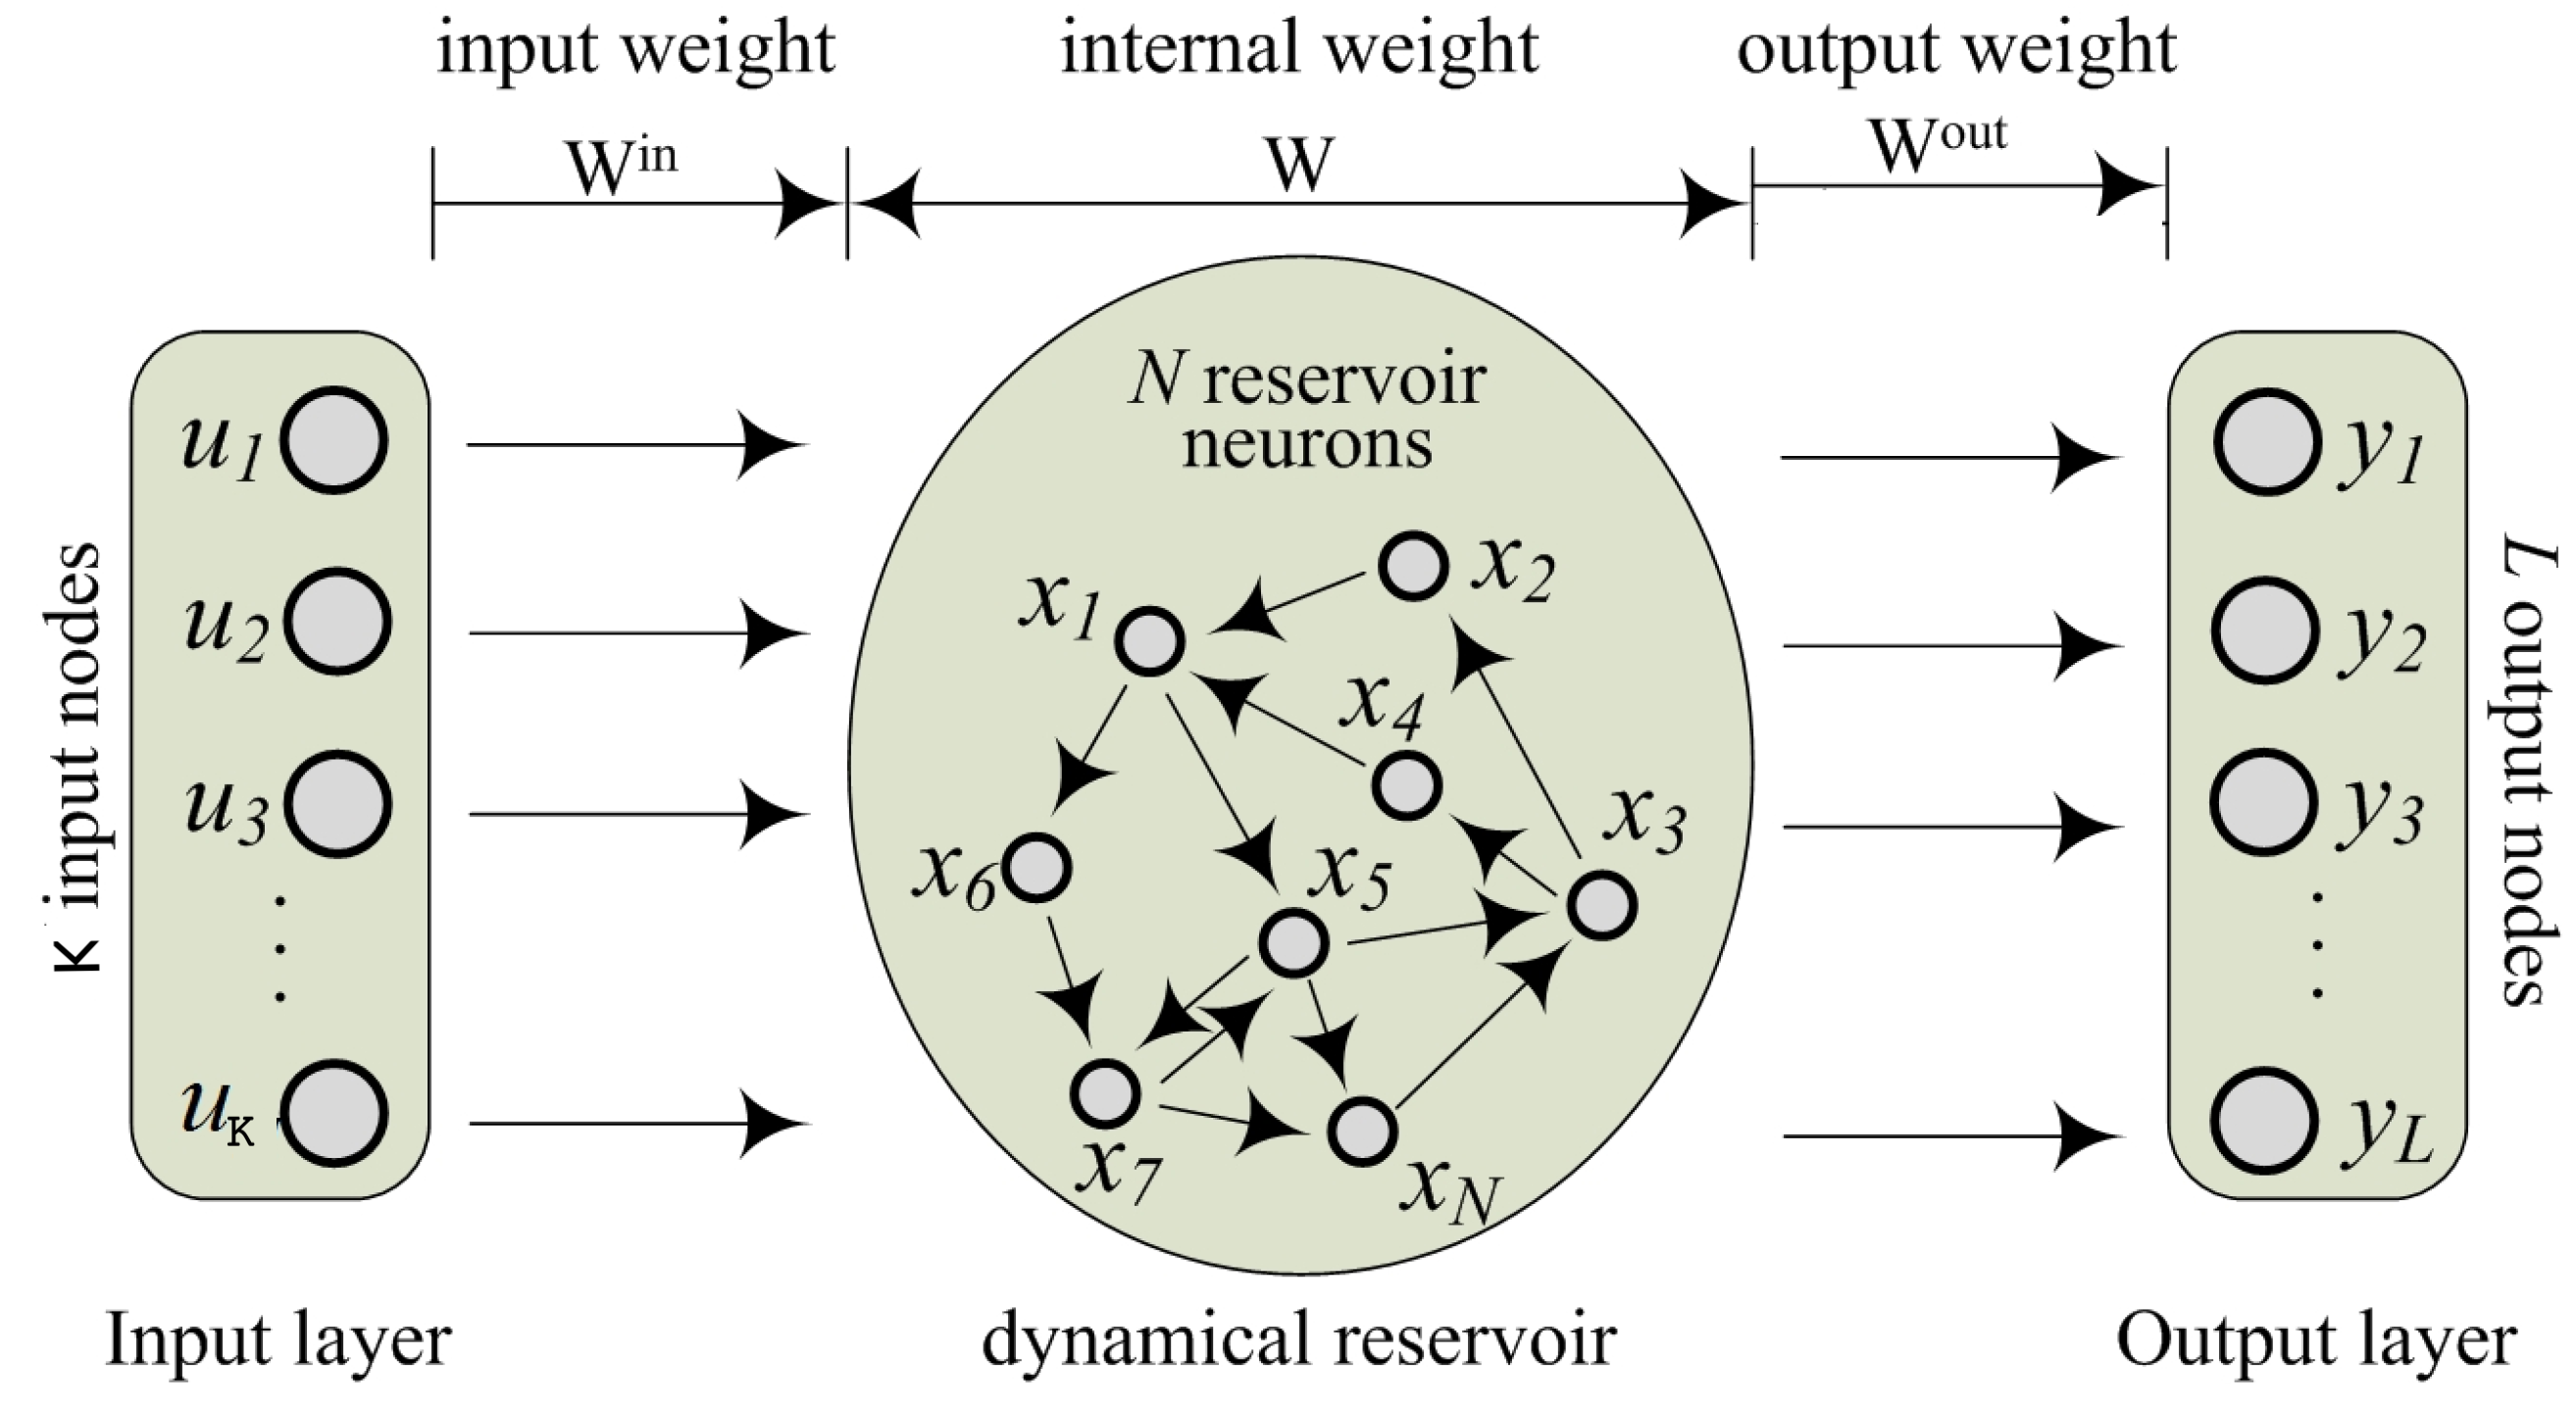
\includegraphics[width = 10cm]{./backgroundConcepts/images/esn1}
	 \caption{The basic schema of Echo State Network. Image source\cite{Li_2015}.}
  \end{figure}
 
 
 
  \subsection{Formalism}
  We consider discrete time neural networks with $K$ input units, $N$ internal network units and $L$ output units. Each of units at time step n has activation. Activations of input units at time step n are $\mathbf{u}(n) = (u_1(n),\hdots,u_K(n))$, of internal units are $\mathbf{x}(n) =( x_1(n),\hdots,x_N(n) )$ and of output units are $\mathbf{y}(b) = (y_1(n),\hdots,y_L(n))$. Real valued connection wights for the input links are collected in the matrix $\mathbf{W}^{in} \in \mathbb{R}^{N \times K }$, for the synaptic links between the neurons in the network are collected in matrix $\mathbf{W} \in \mathbb{R}^{N \times N }$, and for the output weights are collected in matrix $\mathbf{W}^{out} \in \mathbb{R}^{L \times (K+N+L) }$ \cite{EchoStatesTechRep}. The connections from input to output are used and the corresponding connection weights are stored in matrix $\mathbf{W}^{out}$. The output units may optionally project back to internal units with connections however they have not been used in this experiment. A zero weight value can be interpreted as "no connection" \cite{aeger_TrainingRNNsTutorial.2005}. \\
  \indent \indent
  The activation of internal units are updated according to the discrete time state update equation given below:
   %
   \begin{equation} \label{eq:stateUpdate}
    \textbf{x}(n+1) = f(\textbf{Wx}(n) +  \textbf{W}^{in}\textbf{u}(n+1) + \mathbf{B} )
  \end{equation}
   where $\mathbf{u}(n)$ is the externally given input,$f()$ denotes the the component-wise application of unit output function ($tanh$ used for this experiment), and $\mathbf{B} \in \mathbb{R}^N$ is the bias vector .
   %  $\mathbf{x}(n)$ is $N$
  % dimensional state of the network at time point $n$, $\mathbf{W}$ is $N\times N$ matrix
  % consisting the weights of synaptic links connecting the neurons in reservoir, \textbf{W}$^{in}$ is $N\times K$ matrix consisting
  % weights of input links, \textbf{y}(n) is the output signal at time point $n$ and \textbf{B} is the bias vector of dimension $N$.
 
 % For our implementation, we have ignored output feedback to the network so the
 % state equation reduces to
 %  \begin{equation} \label{eq:stateUpdate}
 %   \textbf{x}(n+1) = f(\textbf{Wx}(n) +  \textbf{W}^{in}\textbf{u(n+1)} + \mathbf{B} )
 % \end{equation}

 The extended system state \textbf{z}(n) = [\textbf{x}(n) ; \textbf{u}(n)] is obtained 
 by the concatenation of system states and input signal at time $\mathbf{n}$. For each time point, $i = 1,\hdots ,n_{max}$, the extended system state is stacked row-wise in a state collection matrix \textbf{S}. This process is known as harvesting reservoir state. The output is 
 obtained from the extended system states by the equation below:
 \begin{equation} \label{eq:prediction}
   \mathbf{y}(n) = \mathbf{g}(\mathbf{W}^{out} \mathbf{z}(n) )
 \end{equation}
   % where $\mathbf{W}^{out}$ is $L\times(K+N)$ dimensional matrix of output
%    weights and
   $\mathbf{g} = (g_1, \hdots,g_L)$ is unit output activation function (in our case identity).\cite{Jaeger:2007}.
  
   The $\textbf{W}^{out}$ matrix consisting the weights of links connecting reservoirs to output nodes is obtained by the linear 
   regression of weights of desired outputs \textbf{d}(n) on the harvested 
   extended systems states \textbf{z}(n). \textbf{W}$^{out}$ can be computed 
   efficiently by linear regression of \textbf{S} and \textbf{D} as given by Equation \eqref{eq:wout} .
   \begin{equation}\label{eq:wout}
 	\mathbf{W}^{out} =
      (\mathbf{S^{'}S} + \alpha \mathbf{I})^{-1}\mathbf{SD}^{'}
 	 % \label{eq:linreg}
      \end{equation}
     
      where $\alpha$ is the regularization coefficient \textbf{D} is 
      desired output vector\cite{Jaeger:2007}.